\documentclass[]{article}
\usepackage[latin1]{inputenc}
\usepackage{ragged2e}
\AtBeginDocument{\RaggedRight}
\usepackage{amsmath}
\usepackage{amssymb}
\renewcommand{\labelitemi}{\color{MPIIblue} $\blacktriangleright$}
\usepackage{rotating}
\usepackage{latexsym}
\usepackage{graphicx}
\usepackage{wasysym}
\usepackage{multirow}
\graphicspath{{../Stutz2019CVPR/}}
\usepackage{url}
\usepackage{calc}
\usepackage[
    a4paper,
    left=2.5mm,
    right=2.5mm,
    top=2mm,
    bottom=2mm,
    includehead,
    headheight=17.5mm,
]{geometry}
\usepackage{fancyhdr}
\usepackage{parskip}
\usepackage{tikz}
\usetikzlibrary{math}
\usepackage{tikz-3dplot}
\usepackage{pgfplots}
\usetikzlibrary{calc}
\usetikzlibrary{shadings,shadows}
\usepackage{xcolor}
\usepackage{tcolorbox}
\tcbuselibrary{skins,breakable}
\usepackage[backend=bibtex,style=numeric]{biblatex}

\pagestyle{fancy}
\makeatletter
\def\headrule{}
\def\footrule{}
\makeatother
\lfoot{ %
    %\hspace*{0.5mm}
    %\raisebox{14.5mm}{
\includegraphics[height=14mm]{gfx/mpilogo-inf-narrow}}
}
\cfoot{}
\rfoot{ %
    %\raisebox{16mm}{
\includegraphics[height=12mm]{gfx/UT_WBMW_Rot_RGB}}
}
\lhead{%
	\vspace*{2mm}
    \hspace*{1.5mm}{\bf\Large Bit Error Robustness for\\[2mm]\hspace*{1.5mm}Energy-Efficient DNN Accelerators}\\[3mm]
    \hspace*{1.5mm}{\large David Stutz, Nandhini Chandramoorthy, Matthias Hein, Bernt Schiele}
}
\chead{%
    \hspace*{60mm}\raisebox{6mm}{
\includegraphics[height=10mm]{mpilogo-inf-narrow}}\hspace*{2.5mm}
    \raisebox{7.5mm}{
\includegraphics[height=9mm]{UT_WBMW_Rot_RGB}}
}
\rhead{%
    \raisebox{7.5mm}{
\includegraphics[height=9mm]{IBM_logo_pos_RGB}}
}

\bibliography{bibliography}

\renewcommand{\rmdefault}{phv}
\renewcommand{\sfdefault}{phv}
\renewcommand{\ttdefault}{pcr}

\definecolor{MPIIblue}{RGB}{0,51,93}
\definecolor{MPIIlightblue}{RGB}{103,133,158} % 67859E
\definecolor{MPIIorange}{RGB}{200,91,15} % C85B0F
\definecolor{MPIIblack}{RGB}{46,46,46}
\definecolor{MPIIwhite}{RGB}{255,255,255}
\definecolor{MPIIdarkgray}{RGB}{123,123,123}
\definecolor{MPIIdarkergray}{RGB}{89,89,89}
\definecolor{MPIIgray}{RGB}{169,169,169}
\definecolor{MPIIlightgray}{RGB}{214,214,214}
\definecolor{MPIIlightergray}{RGB}{234,234,234}
\definecolor{MPIIgreen}{HTML}{327a2b} % 0.22,0.54, 0.19
\definecolor{MPIIred}{rgb}{0.65,0.23,0.25}
\definecolor{MPIIbeige}{rgb}{0.65,0.23,0.25}
\definecolor{MPIIpink}{HTML}{d36582}
\definecolor{MPIIteal}{HTML}{4d7c8a}
\definecolor{MPIIviolet}{HTML}{3c1642}
\definecolor{MPIIbrown}{HTML}{5a352a}
\definecolor{MPIIyellow}{HTML}{eee82c}
\definecolor{colorbrewer0}{RGB}{45,45,45}
\definecolor{colorbrewer1}{RGB}{228,26,28}
\definecolor{colorbrewer2}{RGB}{55,126,184}
\definecolor{colorbrewer3}{RGB}{77,175,74}
\definecolor{colorbrewer4}{RGB}{152,78,163}
\definecolor{colorbrewer5}{RGB}{255,127,0}
\definecolor{colorbrewer6}{RGB}{255,255,51}
\definecolor{colorbrewer7}{RGB}{166,86,40}
\definecolor{colorbrewer8}{RGB}{247,129,191}
\definecolor{colorbrewer9}{RGB}{153,153,153}
\definecolor{colorbrewer10}{RGB}{24,167,181}
\pgfplotsset{
	Error/.style={colorbrewer2,line width=1.5pt},
	Energy/.style={colorbrewer5,line width=1.5pt},
	%
	%
	DotNormal/.style={black!25!white,only marks,mark=*,mark size=1.75pt},
	DotClipping/.style={black!25!white,only marks,mark=*,mark size=1.75pt},
	DotRandom/.style={black!25!white,only marks,mark=*,mark size=1.75pt},
    %
    OptNormal/.style={colorbrewer5,solid,line width=2pt,opacity=0.75,solid,mark=*,mark size=2.5pt,mark options={opacity=1}},
    OptQuant/.style={colorbrewer7,solid,line width=2pt,opacity=0.75,solid,mark=*,mark size=2.5pt,mark options={opacity=1}},
    OptClipping/.style={colorbrewer2,solid,line width=2pt,opacity=0.75,mark=*,mark size=2.5pt,mark options={opacity=1}},
    OptRandom/.style={colorbrewer4,solid,line width=2pt,opacity=0.75,mark=*,mark size=2.5pt,mark options={opacity=1}},
    Opt/.style={colorbrewer0,solid,mark=*,mark size=1.5pt,line width=1.25pt},
    Opt05/.style={colorbrewer0,dash pattern={on 7pt off 2pt on 1pt off 3pt},solid,mark=*,mark size=1.5pt,line width=1.25pt},
    Opt2/.style={colorbrewer0,dashed,mark=*,mark size=1.25pt,mark options={solid},line width=1.5pt},
    Opt3/.style={colorbrewer0,dash pattern={on 7pt off 2pt on 1pt off 3pt},mark=*,mark size=1.5pt,mark options={solid},line width=1.25pt},
    Opt4/.style={colorbrewer0,dotted,mark=*,mark size=1.5pt,mark options={solid},line width=1.25pt},
}
\tikzmath
{
		  function symlog(\x,\a){
		    \yLarge = ((\x>\a) - (\x<-\a)) * (ln(max(abs(\x/\a),1)) + 1);
		    \ySmall = (\x >= -\a) * (\x <= \a) * \x / \a ;
		    return \yLarge + \ySmall ;
		  };
		  function symexp(\y,\a){
		    \xLarge = ((\y>1) - (\y<-1)) * \a * exp(abs(\y) - 1) ;
		    \xSmall = (\y>=-1) * (\y<=1) * \a * \y ;
		    return \xLarge + \xSmall ;
		  };
}
\def\basis{0.001}
\pgfplotsset{
	x coord trafo/.code={\pgfmathparse{symlog(#1,\basis)}\pgfmathresult},
	x coord inv trafo/.code={\pgfmathparse{symexp(#1,\basis)}\pgfmathresult},
}

\newenvironment{problem}[1]{%
    \tcolorbox[noparskip,frame hidden,boxrule=0.5mm,colframe=MPIIblue,
    colbacktitle=MPIIblue,coltitle=MPIIwhite,
    colback=MPIIwhite,
    titlerule=0mm,sharpish corners,no shadow,
    left=1.5mm,top=1.5mm,right=1.5mm,bottom=1mm,
    lefttitle=1.5mm,toptitle=2mm,righttitle=1.5mm,bottomtitle=2mm,
    title=#1]}%
{\endtcolorbox}
\newenvironment{related}[1]{%
    \tcolorbox[noparskip,frame hidden,boxrule=0.5mm,colframe=MPIIgray,
    colbacktitle=MPIIgray,coltitle=MPIIwhite,
    colback=MPIIwhite,
    titlerule=0mm,sharpish corners,no shadow,
    left=1.5mm,top=1.5mm,right=1.5mm,bottom=1mm,
    lefttitle=1.5mm,toptitle=2mm,righttitle=1.5mm,bottomtitle=2mm,
    title=#1]}%
{\endtcolorbox}
\newenvironment{method}[1]{%
    \tcolorbox[noparskip,frame hidden,boxrule=0.5mm,colframe=MPIIorange,
    colbacktitle=MPIIorange,coltitle=MPIIwhite,
    colback=MPIIwhite,
    titlerule=0mm,sharpish corners,no shadow,
    left=1.5mm,top=1.5mm,right=1.5mm,bottom=1mm,
    lefttitle=1.5mm,toptitle=2mm,righttitle=1.5mm,bottomtitle=2mm,
    title=#1]}%
{\endtcolorbox}
\newenvironment{data}[1]{%
    \tcolorbox[noparskip,frame hidden,boxrule=0.5mm,colframe=MPIIgray,
    colbacktitle=MPIIgray,coltitle=MPIIwhite,
    colback=MPIIwhite,
    titlerule=0mm,sharpish corners,no shadow,
    left=1.5mm,top=1.5mm,right=1.5mm,bottom=1mm,
    lefttitle=1.5mm,toptitle=2mm,righttitle=1.5mm,bottomtitle=2mm,
    title=#1]}%
{\endtcolorbox}
\newenvironment{results}[1]{%
    \tcolorbox[noparskip,frame hidden,boxrule=0.5mm,colframe=MPIIlightgray,
    colbacktitle=MPIIlightgray,coltitle=MPIIblue,
    colback=MPIIwhite,
    titlerule=0mm,sharpish corners,no shadow,
    left=1.5mm,top=1.5mm,right=1.5mm,bottom=1mm,
    lefttitle=1.5mm,toptitle=1.05mm,righttitle=1.5mm,bottomtitle=1.05mm,
    title=#1]}%
{\endtcolorbox}
\newenvironment{moreresults}[1]{%
	\tcolorbox[noparskip,frame hidden,boxrule=0.5mm,colframe=MPIIlightgray,
	colbacktitle=MPIIwhite,coltitle=MPIIblue,
	colback=MPIIwhite,
	titlerule=0.5mm,sharpish corners,no shadow,
	left=1.5mm,top=1.5mm,right=1.5mm,bottom=1mm,
	lefttitle=1mm,toptitle=0.5mm,righttitle=1mm,bottomtitle=0.25mm,
	title=#1]}%
{\endtcolorbox}
\newenvironment{code}[1]{%
    \tcolorbox[noparskip,frame hidden,boxrule=0mm,colframe=MPIIwhite,
    colback=MPIIorange,coltext=MPIIwhite,
    titlerule=0mm,sharpish corners,no shadow,
    left=2.5mm,top=2.5mm,right=2.5mm,bottom=2.5mm,
    lefttitle=1.5mm,toptitle=2mm,righttitle=1.5mm,bottomtitle=2mm,
    title=#1]}%
{\endtcolorbox}
\newenvironment{references}[1]{%
    \tcolorbox[noparskip,frame hidden,boxrule=0.5mm,colframe=MPIIlightgray,
    colbacktitle=MPIIwhite,coltitle=MPIIdarkergray,
    colback=MPIIwhite,
    titlerule=0mm,sharpish corners,no shadow,
    left=1.5mm,top=0.25mm,right=1.5mm,bottom=0.5mm,
    lefttitle=1.5mm,toptitle=2mm,righttitle=1.5mm,bottomtitle=2mm,
    title=#1]}%
{\endtcolorbox}

\begin{document}
	\vspace*{-10mm}
    \begin{minipage}[t]{0.495\textwidth}
        \strut\vspace*{-\baselineskip} % !
        
        \begin{problem}{\bfseries\large Problem}
        	{\large \textbf{Low-voltage operation} of DNN accelerators to save energy causes \textbf{bit errors} in memory:}
        	\vspace*{1mm}
        	
            \begin{center}
            	\begin{tikzpicture}
       			\begin{axis}[
       					xmin=0.75,
       					xmax=1,
       					ymin=0,
       					ymax=21,
       					ymode=log,
       					grid=both,
       					grid style={line width=.1pt, draw=gray!25},
       					major grid style={line width=.2pt,draw=gray!50},
       					minor tick num=1,
       					width=8cm,
       					height=6cm,
       					ytick={0.0001, 0.001, 0.01, 0.1, 1, 2.5, 10, 20},
       					yticklabels={$10^{-4}$, $10^{-3}$, $10^{-2}$, $10^{-1}$, 1, \raisebox{2px}{2.5}, \raisebox{-8px}{10}, \raisebox{4px}{20}},
       					xticklabel style={/pgf/number format/precision=2,/pgf/number format/fixed},
       					scaled x ticks=false,
       					yticklabel style={/pgf/number format/precision=2,/pgf/number format/fixed},
       					scaled y ticks=false,
       					ylabel=Bit Error Rate $p$ in \%,
       					y label style={at={(axis description cs:0.05,0.5)},anchor=south,font=\large},
       					xlabel={Supply Voltage, Normalized by $V_{\text{min}}$},
       					x label style={at={(axis description cs:0.5,0.02)},anchor=north,font=\large},
       				]
       				
       				\addplot[Error] coordinates {
       					(0.75, 20.56)
       					(0.792, 5.573)
       					(0.833, 1.115)
       					(0.875, 0.129)
       					(0.917, 0.00686646)
       					(0.958, 0.000190735)
       					(1.0, 0)
       				};\label{plot:error}
       				\end{axis}
       				\begin{axis}[
       				axis y line*=right,
       				xmin=0.75,
       				xmax=1,
       				ymax=1.03,
       				ymin=0.48,
       				xtick={},
       				ytick={0.6, 0.8, 1},
       				xticklabels={},
       				width=8cm,
       				height=6cm,
       				ylabel=\begin{tabular}{c}Normalized Energy\\per SRAM Access\end{tabular},
       				y label style={at={(axis description cs:1.275,0.5)},anchor=north,font=\large},
       				legend style={fill=white, fill opacity=0.6, draw opacity=1,text opacity=1,at={(axis description cs:0.13,0.01)},anchor=south west,row sep=-2.5pt,font=\large,/tikz/every even column/.append style={row sep=0.25cm}},
       				legend cell align={left},
       				]
       				\addlegendimage{/pgfplots/refstyle=plot:error}\addlegendentry{Bit Error Rate $p$};
       				\addplot[Energy] coordinates {
       					(0.75, 0.5625)
       					(0.792, 0.626736111)
       					(0.833, 0.694444444)
       					(0.875, 0.765625)
       					(0.917, 0.840277778)
       					(0.958, 0.918402778)
       					(1.0, 1)
       				};
       				\addlegendentry{Normalized Energy};
       				\coordinate (Vmin) at (axis cs:1,0.485) {};
					\coordinate (v2) at (axis cs:0.833, 0.694444444) {};
					\coordinate (v3) at (axis cs:0.875, 0.765625) {};
       				\end{axis}
       				\node[anchor=north west,yshift=-0.4mm] at (Vmin){\small ${=}V_{\text{min}}$};
       				\node[anchor=north west,yshift=-0.4mm] at (Vmin){\small ${=}V_{\text{min}}$};
					\node[anchor=south east,draw=black,inner sep=0.25pt,line width=1pt,xshift=-0.15cm,fill=white,fill opacity=0.6,text opacity=1] at (v2) {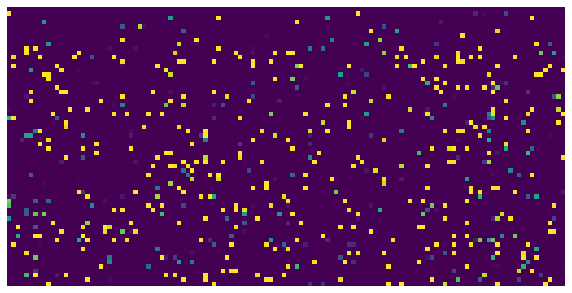
\includegraphics[height=1.125cm]{../talk/gfx/18_2}};
					\node[anchor=north west,draw=black,inner sep=0.25pt,line width=1pt,xshift=0.15cm,fill=white,fill opacity=0.6,text opacity=1] at (v3) {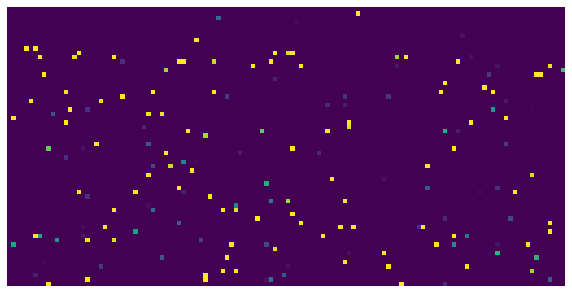
\includegraphics[height=1.125cm]{../talk/gfx/18_3}};
					\draw[line width=1pt] (v2) circle(3pt);
					\draw[-,line width=1pt] ($(v2) + (0,0.1)$) -- ($(v2) + (0,1.05)$) -- ($(v2) + (-0.175,1.05)$);
					\draw[line width=1pt] (v3) circle(3pt);
					\draw[-,line width=1pt] ($(v3) + (0,-0.1)$) -- ($(v3) - (0,1.05)$) -- ($(v3) - (-0.175,1.05)$);
       			\end{tikzpicture}
            \end{center}
        \end{problem}
        
        \begin{method}{\bfseries\large Contributions}
        	%\vspace*{-2.5mm}
        	
        	{\large
        		\textbf{Improve bit error robustness} of DNNs:\\[1mm]
	       		{\fcolorbox{MPIIblue}{MPIIblue}{\hskip 0.02cm\color{MPIIwhite}1\hskip 0.02cm}} Robust fixed-point quantization (\textsc{RQuant} \ref{quant}).\\[0.5mm]
	       		{\fcolorbox{MPIIblue}{MPIIblue}{\hskip 0.02cm\color{MPIIwhite}2\hskip 0.02cm}} Weight clipping regularization (\textsc{Clipping} \ref{clipping}).\\[0.5mm]
	       		{\fcolorbox{MPIIblue}{MPIIblue}{\hskip 0.02cm\color{MPIIwhite}3\hskip 0.02cm}} Random bit error training (\textsc{RandBET} \ref{random}).
       		}
       		\vspace*{2.5mm}
       		
            \begin{center}
	            \begin{tikzpicture}
	       		\begin{axis}[
	       				ymin=4.3,
	       				ymax=8,
	       				xmin=0,
	       				xmax=3,
	       				xtick={0, 0.01, 0.05, 0.1, 0.5, 1, 2.5},
	       				xticklabels={$0$, $0.01$, $0.05$, $0.1$, $0.5$, $1$, $2.5$},
	       				ytick={4.3, 5, 6, 7, 8, 9, 10},
	       				scaled x ticks=false,
	       				xticklabel style={/pgf/number format/precision=2,/pgf/number format/fixed},
	       				scaled y ticks=false,
	       				yticklabel style={/pgf/number format/precision=2,/pgf/number format/fixed},
	       				log ticks with fixed point,
	       				grid=major,
	       				xlabel={Bit Error Rate $p$ (\%)},
	       				ylabel={Robust Test Error RErr (\%)},
	       				x label style={at={(axis description cs:0.5,0.03)},anchor=north,font=\large},
	       				y label style={xshift=-2mm,at={(axis description cs:0.09,0.5)},anchor=south,font=\large},
	       				width=9cm,
	       				height=6cm,
	       				legend style={at={(axis description cs:0.02,0.98)},anchor=north west,font=\small,fill opacity=0.4,text opacity=1},
	       				legend cell align={left},
	       			]
	       			
	       			\addplot[OptNormal] coordinates {
	       			(0.0, 4.36) % 0.0
	       			(0.005, 4.71) % 0.005
	       			(0.01, 4.82) % 0.01
	       			(0.025, 5.09) % 0.025
	       			(0.05, 5.510000000000001) % 0.05
	       			(0.075, 5.949999999999999) % 0.075
	       			(0.1, 6.370000000000001) % 0.1
	       			(0.25, 10.190000000000001) % 0.25
	       			(0.5, 24.759999999999998) % 0.5
	       			(0.75, 50.1) % 0.75
	       			(1.0, 72.65) % 1.0
	       			(1.5, 87.4) % 1.5
	       			(2.0, 89.75999999999999) % 2.0
	       			(2.5, 90.14999999999999) % 2.5
	       			};
	       			\label{normal}
	       			\addplot[OptQuant] coordinates {
	       			(0.0, 4.32)
	       			(0.005, 4.52)
	       			(0.01, 4.6)
	       			(0.025, 4.83)
	       			(0.05, 5.1)
	       			(0.075, 5.3100000000000005)
	       			(0.1, 5.54)
	       			(0.25, 7.08)
	       			(0.5, 11.28)
	       			(0.75, 18.44)
	       			(1.0, 32.05)
	       			(1.5, 68.65)
	       			(2.0, 85.28)
	       			(2.5, 89.01)
	       			};
	       			\label{quant}
	       			\addplot[OptClipping] coordinates {
	       			(0.0, 4.42)
	       			(0.005, 4.569999999999999)
	       			(0.01, 4.66)
	       			(0.025, 4.81)
	       			(0.05, 5.01)
	       			(0.075, 5.16)
	       			(0.1, 5.3100000000000005)
	       			(0.25, 6.17)
	       			(0.5, 6.529999999999999)
	       			(0.75, 6.8500000000000005)
	       			(1.0, 7.180000000000001)
	       			(1.5, 7.920000000000001)
	       			(2.0, 8.7)
	       			(2.5, 9.02)
	       			};
	       			\label{clipping}
	       			\addplot[OptRandom] coordinates {
	       			(0.0, 4.44)
	       			(0.005, 4.65)
	       			(0.01, 4.67)
	       			(0.025, 4.8500000000000005)
	       			(0.05, 5.07)
	       			(0.075, 5.24)
	       			(0.1, 5.37)
	       			(0.25, 5.81)
	       			(0.5, 6.18)
	       			(0.75, 6.47)
	       			(1.0, 6.710000000000001)
	       			(1.5, 7.13)
	       			(2.0, 7.580000000000001)
	       			(2.5, 8.02)
	       			};
	       			\label{random}
	       			\addplot[Opt] coordinates {
	       			(0.0, 4.32)
	       			(0.005, 4.52)
	       			(0.01, 4.6)
	       			(0.025, 4.81)
	       			(0.05, 5.01)
	       			(0.075, 5.16)
	       			(0.1, 5.3100000000000005)
	       			(0.25, 5.81)
	       			(0.5, 6.18)
	       			(0.75, 6.47)
	       			(1.0, 6.710000000000001)
	       			(1.5, 7.13)
	       			(2.0, 7.580000000000001)
	       			(2.5, 8.02)
	       			};
	       			\label{opt}
	       			\addplot[Opt2] coordinates {
	       			(0.0, 4.5)
	       			(0.005, 4.65)
	       			(0.01, 4.72)
	       			(0.025, 4.89)
	       			(0.05, 5.050000000000001)
	       			(0.075, 5.220000000000001)
	       			(0.1, 5.36)
	       			(0.25, 5.94)
	       			(0.5, 6.38)
	       			(0.75, 6.68)
	       			(1.0, 6.98)
	       			(1.5, 7.51)
	       			(2.0, 8.06)
	       			(2.5, 8.62)
	       			};
	       			\label{opt2}
	       			\end{axis}
	       			\node [draw,fill=white,text opacity=1,fill opacity=0.5,anchor=north west] at (rel axis cs: 0.02, 0.98) {\shortstack[l]{
	       			\underline{$8$ Bit Quant.:}\\
	       			\ref{normal} \textsc{Normal}\\[1px]
	       			\ref{quant} \textsc{RQuant}\\
	       			\ref{clipping} +\textsc{Clipping}\\[1px]
	       			\ref{random} +\textsc{RandBET}}};
	       			\node [draw,fill=white,text opacity=1,fill opacity=0.5,anchor=south east] at (rel axis cs: 0.98, 0.02) {\shortstack[l]{
	       			\ref{opt} Best, $8$ bits\\
	       			\ref{opt2} Best, $4$ bits}};
	       		\end{tikzpicture}
       		\end{center}
        \end{method}
    
        \vspace*{-2mm}
        \begin{minipage}[t]{\textwidth}
            \strut\vspace*{-\baselineskip} % !
            
            \begin{code}{}
                \large
                Paper and Code: \bf\url{davidstutz.de/randbet}
            \end{code}
        \end{minipage}
   
        \vspace*{-1mm}
   		\begin{data}{\bfseries\large Bit Error Model}
   			\vspace*{-3mm}
   			\begin{center}
   				\hspace*{-3.5mm}
				\begin{tikzpicture}
					\node[anchor=north west] at (-0.25,1.75){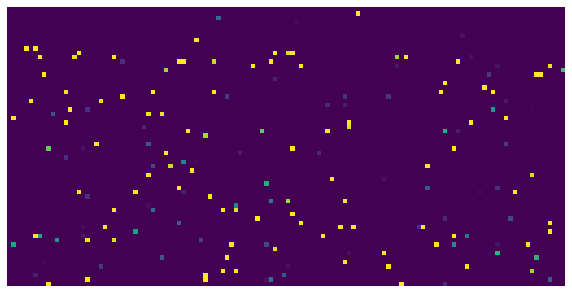
\includegraphics[width=4.9cm,trim={0 4cm 0 0},clip]{../talk/gfx/18_3}};
					\node[anchor=north west] at (4.65,1.75){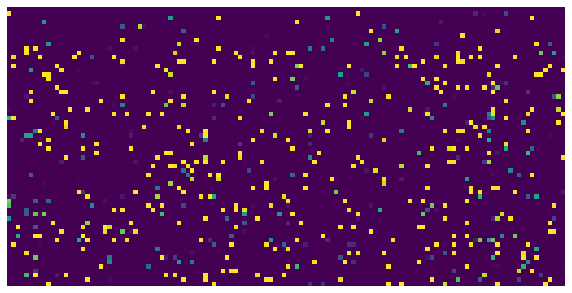
\includegraphics[width=4.9cm,trim={0 4cm 0 0},clip]{../talk/gfx/18_2}};
					\draw[line width=1pt,-] (2.25,1.6) -- (2.25,1.85) -- (4,1.85);
					\draw[line width=1pt,-] (5.75,1.85) -- (7.5,1.85) -- (7.5,1.6);
					\node at (4.9,1.85){\normalsize subset of};
					\node[anchor=north west,fill=white,fill opacity=0.6,text opacity=1,inner sep=2.5pt] at (0.05, 1.45){\normalsize $p{\approx}0.86\%$};
					\node[anchor=north west,fill=white,fill opacity=0.6,text opacity=1,inner sep=2.5pt] at (4.95, 1.45){\normalsize $p{\approx}2.75\%$};
				\end{tikzpicture}
			\end{center}
			
			{\large {\color{MPIIblue}$\RHD$} Uniform random bit errors (across loc. \& chips).}
		\end{data}
   
        \vspace*{-1mm}
        \begin{related}{\bfseries\large Related Work}
            \large 
           	{\color{MPIIblue}$\RHD$} \cite{MurthyARXIV2019,MerollaARXIV2016,SungARXIV2015} DNN robustness \emph{to} quantization errors\\[1mm]
           	{\color{MPIIblue}$\RHD$} \cite{KimDATE2018,KoppulaMICRO2019} training on \emph{profiled} bit errors, fixed patterns
        \end{related}
    \end{minipage}
    \hfill
    \begin{minipage}[t]{0.495\textwidth}
        \strut\vspace*{-\baselineskip} % !
        
        \begin{results}{\bf\large\fcolorbox{MPIIblue}{MPIIblue}{\hskip 0.05cm\color{MPIIwhite}1\hskip 0.05cm} Robust Quantization (\textsc{RQuant})}
        	{\large 
	            Simple fixed-point quantization scheme:
	       		\begin{align*}
	       			Q(w_i) = \left\lfloor\frac{w_i}{\Delta}\right\rfloor, Q^{-1}(v_i) = \Delta v_i, \Delta = \frac{q_{\text{max}}}{w^{m - 1} - 1}\notag
	       		\end{align*}
	       		\vspace*{-0.5cm}
	       		\begin{itemize}
	       			\item weight $w_i \in [-q_{\text{max}}, q_{\text{max}}]$, $m$ bits (e.g., $m = 8$)
	       		\end{itemize}
       		}
       		\vspace*{1mm}
        \end{results}
        
        \vspace*{-1mm}
        \begin{minipage}[t]{0.4975\textwidth}
    		\begin{moreresults}{Bit errors and quantization:}
               	\vspace*{-2mm}
               	\begin{center}
               		\hspace*{-4mm}
           			\resizebox{1.125\textwidth}{!}{
           			\begin{tikzpicture}
       					\node[anchor=north west] at (-0.25,0){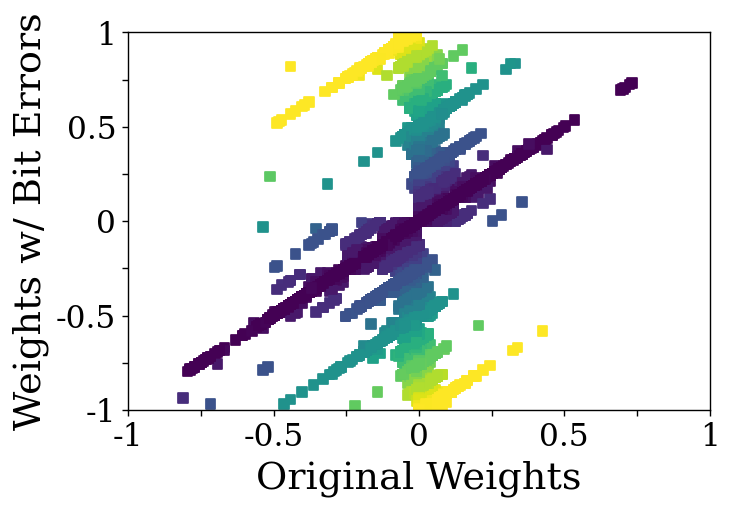
\includegraphics[height=3cm]{../paper/c10_errors_q81unfp_nt.png}};
       					\node[anchor=north west] at (4,0){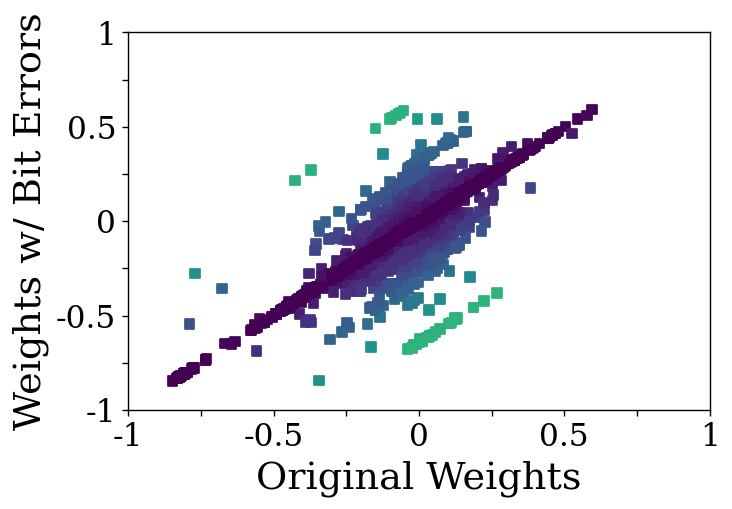
\includegraphics[height=3cm,trim=1cm 0 0 0,clip]{../paper/c10_errors_q81auunfp_nt.png}};
       					
       					\node[anchor=south,xshift=0.25cm,yshift=-0.25cm] at (2, 0){\textbf{Global}, $q_{\text{max}}=1$};
       					\node[anchor=south,xshift=0.25cm,yshift=-0.25cm] at (6, 0){\textbf{Per-Layer{\color{red}+}Asymmetric}};
       				\end{tikzpicture} 
       				}
          		\end{center}
      			\vspace*{-1mm}
            \end{moreresults}
        \end{minipage}
        \begin{minipage}[t]{0.4975\textwidth}
        	\begin{moreresults}{Robustness \& details\vphantom{q}:}
        		\footnotesize
   				\vspace*{-2mm}
   				\hspace*{-2.5mm}
				\begin{tabular}{|@{\hspace*{1mm}}c@{\hspace*{1mm}}|@{\hspace*{1mm}}l@{\hspace*{1mm}}|@{\hspace*{1mm}}c@{\hspace*{1mm}}|@{\hspace*{1mm}}c@{\hspace*{1mm}}|}
					\hline
					& Quantization & \multirow{2}{*}{\begin{tabular}{@{}c@{}}Err\\in \%\end{tabular}} & \multirow{2}{*}{\begin{tabular}{@{}c@{}}RErr\\in \%\end{tabular}}\\
					& {\scriptsize (CIFAR-10, $p = 0.5\%$)} &&\\
					\hline
					\hline
					\multirow{4}{*}{\rotatebox{90}{$8$ bit}} & Per-layer & 4.36 & 24.76\\
					& +asymmetric & 4.36 & {\color{colorbrewer1}40.78}\\
					& +unsigned & 4.42 & 17.00\\
					& +rounding & 4.32 & \bfseries 11.28\\
					\hline
				\end{tabular}
   				\vspace*{-1.7mm}
   			\end{moreresults}
        \end{minipage}
        
        \vspace*{-1mm}
        \begin{results}{\bf\large\fcolorbox{MPIIblue}{MPIIblue}{\hskip 0.05cm\color{MPIIwhite}2\hskip 0.05cm} Weight Clipping (\textsc{Clipping})}
        	\large 
            = clipping weights to $[-q_{\text{max}}, w_{\text{max}}]$ during training.\\[1mm]
  			\begin{itemize}
	  			\item $w_{\text{max}} \neq q_{\text{max}}$, but $q_{\text{max}} \leq w_{\text{max}}$\\[1mm]
	  			\item Does \emph{not} impact \emph{relative} errors!
  			\end{itemize}
        \end{results}
        
        \vspace*{-1mm}
		\begin{minipage}[t]{0.565\textwidth}
			\begin{moreresults}{Understanding weight clipping:}
				\vspace*{-1mm}
				\begin{center}
					\hspace*{-0.4cm}
					\begin{minipage}[t]{0.53\textwidth}
						\vspace*{1px}
						
						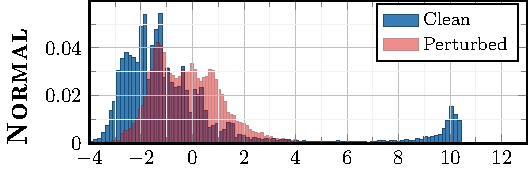
\includegraphics[height=0.9cm]{../paper/c10_q81auunfp_nt_original_logits.pdf}
					\end{minipage}
					\begin{minipage}[t]{0.25\textwidth}
						\vspace*{0px}
						
						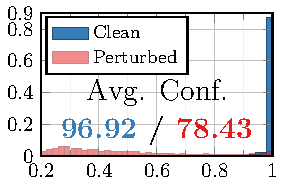
\includegraphics[height=0.9cm]{../paper/c10_q81auunfp_nt_original_confidences.pdf}
					\end{minipage}
					\begin{minipage}[t]{0.22\textwidth}
						\vspace*{0px}
						
						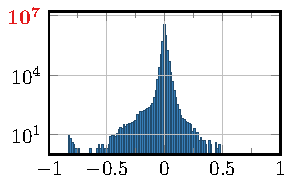
\includegraphics[height=0.9cm]{../paper/c10_q81auunfp_nt_original_weights.pdf}
					\end{minipage}
					
					\hspace*{-0.4cm}
					\begin{minipage}[t]{0.53\textwidth}
						\vspace*{1px}
						
						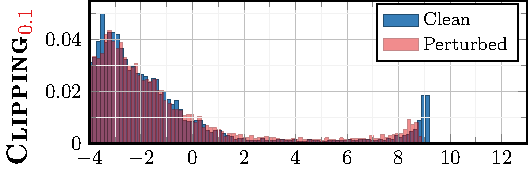
\includegraphics[height=0.9cm]{../paper/c10_q801auunfp_nt_original_logits.pdf}
					\end{minipage}
					\begin{minipage}[t]{0.25\textwidth}
						\vspace*{0px}
						
						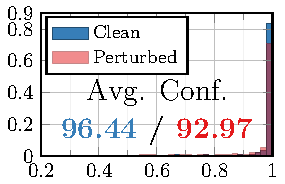
\includegraphics[height=0.9cm]{../paper/c10_q801auunfp_nt_original_confidences.pdf}
					\end{minipage}
					\begin{minipage}[t]{0.22\textwidth}
						\vspace*{0px}
						
						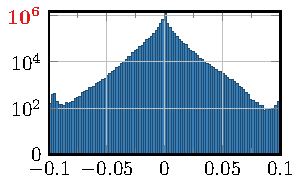
\includegraphics[height=0.9cm]{../paper/c10_q801auunfp_nt_original_weights.pdf}
					\end{minipage}
				\end{center}
				\vspace*{-0.4mm}
			\end{moreresults}
		\end{minipage}
		\begin{minipage}[t]{0.425\textwidth}
			\begin{moreresults}{Robustness:\vphantom{pg}}
				\footnotesize
				\vspace*{-2mm}
   				\hspace*{-2.5mm}
				\begin{tabular}{|@{\hspace*{1mm}}l@{\hspace*{1mm}}|@{\hspace*{1mm}}c@{\hspace*{1mm}}|@{\hspace*{1mm}}c@{\hspace*{1mm}}|}
					\hline
					Model & \multirow{2}{*}{\begin{tabular}{@{}c@{}}Err\\in \%\end{tabular}} & \multirow{2}{*}{\begin{tabular}{@{}c@{}}RErr\\in \%\end{tabular}}\\
					{\scriptsize (CIFAR-10, $p{=}1\%$)} &&\\
					\hline 
					\hline
					\textsc{RQuant} & \bfseries 4.32 & 32.05\\
					\hline
					\textsc{Clipping}\textsubscript{$0.15$} & 4.42 & 13.08\\
					\textsc{Clipping}\textsubscript{$0.05$} & 5.44 & \bfseries 7.18\\
					\hline
					\textsc{Clipping}\textsubscript{$0.15$}+LS & 4.67 & {\color{colorbrewer1}29.40}\\
					\hline
				\end{tabular}
				\vspace*{-2mm}
			\end{moreresults}
		\end{minipage}
        
        \vspace*{-1mm}
        \begin{results}{\bf\large\fcolorbox{MPIIblue}{MPIIblue}{\hskip 0.05cm\color{MPIIwhite}3\hskip 0.05cm} Random Bit Error Training (\textsc{RandBET})}
	        \large 
        	= training on random bit errors.
        	\vspace*{2mm}
            \begin{center}
       			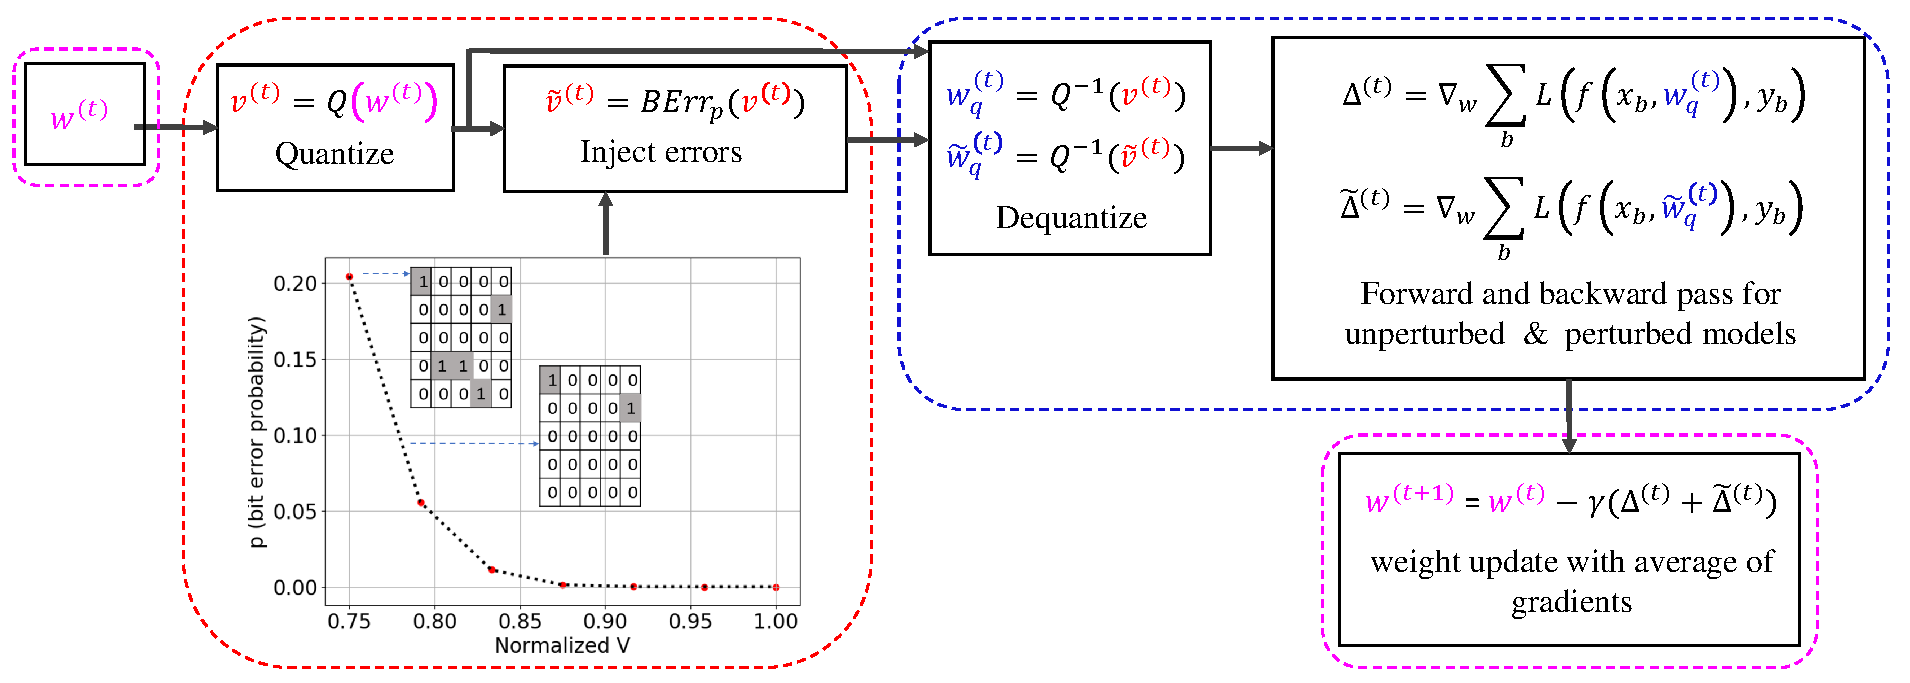
\includegraphics[width=\textwidth]{../paper/main_training_flow4}
       		\end{center}
        \end{results}
        
		\vspace*{-1mm}
		\begin{minipage}[t]{0.505\textwidth}
			\begin{moreresults}{Training on \emph{fixed} bit errors:}
				\footnotesize
				\vspace*{-1mm}
				\hspace*{-2mm}
				\begin{tabular}{|@{\hspace*{1mm}}l@{\hspace*{1mm}}|@{\hspace*{1mm}}c@{\hspace*{1mm}}|@{\hspace*{1mm}}c@{\hspace*{1mm}}|}
					\hline
					Model {\scriptsize(CIFAR-10)} & \multicolumn{2}{@{\hspace*{1mm}}c@{\hspace*{1mm}}|}{RErr in \%}\\
					\hline
					\hline
					\textbf{Fixed Pattern} & $p{=}1$ & $p{=}2.5$\\
					\hline
					Fixed Pattern, $p{=}2.5$ & {\color{colorbrewer1}14.14} & 7.87\\
					+\textsc{Clipping}\textsubscript{$0.15$} & {\color{colorbrewer1}8.50} & 7.41\\
					\hline\hline
					\textbf{\emph{Random} Patterns} & $p{=}1$ & $p{=}2.5$\\
					\hline
					+\textsc{Clipping}\textsubscript{$0.15$} $p{=}2.5$ & 12.09 & 61.59\\
					\hline
				\end{tabular} 
				\vspace*{-1mm}
			\end{moreresults}
		\end{minipage}
		\begin{minipage}[t]{0.485\textwidth}
			\begin{moreresults}{Gen. to \emph{profiled} bit errors:}
				\footnotesize
				\vspace*{-1mm}
				\hspace*{-2mm}
				\begin{tabular}{|@{\hspace*{1mm}}l@{\hspace*{1mm}}|@{\hspace*{1mm}}c@{\hspace*{1mm}}|@{\hspace*{1mm}}c@{\hspace*{1mm}}|}
					\hline
					Model {\scriptsize(CIFAR-10)}& \multicolumn{2}{c|}{RErr in \%}\\
					\hline
					\hline
					\bfseries Chip 1& $p{\approx}0.86$ & {\color{colorbrewer1}$p{\approx}2.75$}\\
					\hline
					\textsc{RandBET}\textsubscript{$0.05$} & 7.04 & 9.37\\
					\hline
					\hline
					\bfseries Chip 2 & $p{\approx}0.14$ & {\color{colorbrewer1}$p{\approx}1.08$}\\
					\hline
					\textsc{RandBET}\textsubscript{$0.05$} & 6.00 & 9.00\\
					\hline
				\end{tabular}
				\vspace*{2.35mm}
			\end{moreresults}
		\end{minipage}
		        
        \vspace*{-1mm}
        \begin{references}{}
            \vspace*{0.325mm}
            \AtNextBibliography{\fontsize{7}{9}\selectfont}
            {\begingroup
                \color{MPIIdarkergray}
                \renewcommand{\section}[2]{}%
                \printbibliography
                \endgroup}
        \end{references}
    \end{minipage}
\end{document}
